\documentclass[11pt,oneside]{article}
\usepackage[T1]{fontenc}
\usepackage[utf8]{inputenc}
\usepackage{tgpagella,tgheros}
\usepackage[letterpaper,margin=0.86in,headheight=15pt,headsep=17pt]{geometry}
\usepackage{amsmath,amssymb,amsthm,mathtools}
\usepackage{graphicx,booktabs,longtable,array,tabularx,microtype,xcolor,float}
\usepackage{enumitem,fancyhdr,needspace,tocloft,hyperref}
\setlength{\cftbeforesecskip}{2pt}\setlength{\cftbeforepartskip}{7pt}
\definecolor{Ink}{HTML}{203D37}
\definecolor{Muted}{HTML}{50605C}
\hypersetup{hidelinks,pdftitle={Machine-Native Reasoning: Connected Synthesis},pdfauthor={Komorebi P.},pdfsubject={Operation Komorebi machine theory compilation, collection edition 1.0.0}}
\pagestyle{fancy}\fancyhf{}
\fancyhead[L]{\small\scshape Machine-Native Reasoning}
\fancyhead[R]{\small Connected synthesis}
\fancyfoot[L]{\scriptsize OPERATION KOMOREBI}
\fancyfoot[R]{\small\thepage}
\renewcommand{\headrulewidth}{0.3pt}
\setlength{\parindent}{0pt}\setlength{\parskip}{5pt}
\setlength{\emergencystretch}{2.5em}
\setcounter{tocdepth}{1}
\newcolumntype{Y}{>{\raggedright\arraybackslash}X}
\newcommand{\src}[1]{\hyperlink{cat:#1}{\textsf{[#1]}}}
\newcommand{\sources}[1]{\par\smallskip{\small\textit{Source route.} #1}\par}
\newcommand{\boundary}[1]{\par\smallskip\noindent\textbf{Boundary.} #1\par}
\newcommand{\parthead}[2]{\clearpage\phantomsection\addcontentsline{toc}{part}{#1: #2}\noindent{\sffamily\small\color{Muted}#1}\par\vspace{4pt}{\sffamily\Large\bfseries\color{Ink}#2}\par\vspace{10pt}}
\newtheorem{connection}{Connecting result}
\newtheorem{example}{Connecting example}
\newtheorem{obstruction}{Obstruction}
\newcommand{\F}{\mathbb F}
\newcommand{\TV}{d_{\mathrm{TV}}}
\newcommand{\im}{\operatorname{im}}
\newcommand{\kerop}{\operatorname{ker}}
\begin{document}
\begin{titlepage}
\thispagestyle{empty}
{\sffamily\small\color{Ink}OPERATION KOMOREBI\hfill REALIZATION CALCULUS}\par
\vspace{0.95in}
{\sffamily\fontsize{35}{39}\selectfont\bfseries\color{Ink}Machine-Native\\Reasoning\par}
\vspace{0.22in}
{\fontsize{21}{27}\selectfont Representation, Learning,\\and Computational Organization\par}
\vspace{0.36in}
{\large A connected compilation of the machine-theory program\par}
\vspace{0.20in}\rule{\linewidth}{0.6pt}
\vspace{0.15in}
\begin{tabularx}{\linewidth}{@{}X>{\raggedleft\arraybackslash}X@{}}
\textbf{Komorebi P.} & Collection edition 1.0.0\\
9 October 2026 & Connected synthesis and source reader
\end{tabularx}
\vfill
\begin{minipage}{0.94\linewidth}\raggedright
\large What a representation preserves. What an operation means. What evidence permits a correction. What a revision costs. What a community can maintain together.
\end{minipage}\par
\vspace{0.6in}
{\small This editorial volume connects twenty-four selected source documents. The source reader preserves their pages and their distinct mathematical, implementation, and research boundaries. A collection of compatible ideas is not, by itself, an implemented general intelligence.}
\end{titlepage}
\pagenumbering{roman}
{\small\setlength{\parskip}{0pt}\tableofcontents}
\clearpage
\section*{How to use this compilation}
\addcontentsline{toc}{section}{How to use this compilation}
This collection has two complementary purposes. The first is to make the machine-related work intelligible as one research program. The second is to retain the actual mathematical sources, rather than replace a substantial body of work with a short architectural summary.

The connected synthesis is a new editorial argument. It introduces a shared vocabulary, a source-to-source interface register, and a small exact example that follows evidence through representation, action, correction, communication, and revision. The twenty-four source documents then supply the detailed proofs, developments, historical boundaries, formal companions, and visual material. Source editions are not renumbered as though they were newly proved chapters of one formal system.

\textbf{There are three reading depths.} Begin with this synthesis for the organizing questions. Read the core machine-theory volume for the recent books together with the signal, language, inference, and mathematical-memory work. Consult the foundations and companion volumes for the extended representation calculus, relational workspace monograph, architecture, formal guides, visual plates, and historical recursive-improvement lineage.

References such as \src{GA} identify a source edition in the catalogue at the end of this synthesis. Its section titles are the preferred locations when source pagination differs from the global reader. The complete compilation adds a source-entry page, an exact page crosswalk, and PDF bookmarks. The original pagination remains visible. A source-page label such as \texttt{GA-8} means physical page eight of that source, including its cover and preliminary pages.

\textbf{The compilation is theory-first.} Its central conclusions depend on explicit mathematical hypotheses. Small exact calculations check the new connecting example and the assembly. No new neural training, broad agent benchmark, hardware run, or corpus-wide Lean rebuild was performed. Some unabridged source works contain retained experimental history. Those pages remain identifiable historical material, not evidence that the entire proposed architecture has been realized.

The collection includes the latest selected Large Signal Model foundations edition recovered for this assembly, 0.4.0, alongside its unchanged software-version boundary. The four recent books retain their first editions. Older long-form theories remain independent sources because their scope is not exhausted by the newer books. \src{LSM}\src{GA}\src{MU}\src{SII}\src{MS}\src{SRWT}\src{SRIC}

\textbf{What this edition does not claim.} It is not an exhaustive census of every machine-related archive in Operation Komorebi. The selected full texts, the six included source archives, and the branches represented only by a source note are listed explicitly. Compilation does not establish historical priority, transfer a proof-assistant guarantee to an unverified implementation, resolve an open learning bridge, or authorize external action.

\clearpage\pagenumbering{arabic}
\parthead{PART I}{One program, several distinct objects}
\section{The unifying question}
A useful machine representation is more than a place to store a correct answer. It enables some future operations and excludes others. It may preserve a probability update while losing the evidence needed to challenge that update. It may predict an output without reconstructing the underlying state. It may express a valid operation while leaving its actual acquisition prohibitively expensive. It may be shared among several agents without creating one collective decision maker.

The central question of this compilation is therefore not whether all these systems are secretly the same object. It is whether their relationships can be made explicit enough that a claim survives the passage from one representation, process, or institution to another.

The strongest common thread is a discipline of \emph{preservation under declared change}. What must remain true when coordinates change? When an observation is compressed? When a learner installs a new operator? When a solver becomes a recipient of another system's explanation? When an institution changes its members or its rules? The answer differs across these cases, but the need to specify it is common.

This perspective organizes the source works without erasing their differences. Grounded Abstraction studies what evidence justifies. Machine Understanding studies what a usable representation enables. Large Signal Model Foundations studies coherent signal realizations, predictive closure, and admissible probability domains. OSL concerns explicit executable semantics. Neuralese concerns latent operations and continuation. AVOC concerns the value and admissibility of computational artifacts. Proof Path Theory concerns the information surrounding a proof. Self-Improving Intelligence concerns changes to discovery procedures. SRWT and Machine Societies concern relational and institutional organization. \src{GA}\src{MU}\src{LSM}\src{OSL}\src{NEU}\src{AVOC}\src{PPT}\src{SII}\src{SRWT}\src{MS}

A compilation becomes misleading when it treats those descriptions as modules already connected by an implemented interface. An equation describing a desirable semantic relation is not the trained translator that realizes it. A defined resource ledger is not evidence that every implementation cost has been metered. A theory of institutions is not evidence that institutions have formed spontaneously.

The positive aim is more precise: build a map of the mathematical objects that can be composed, the assumptions that composition consumes, the obstructions that prevent it, and the information that must remain available for future correction.

\needspace{17\baselineskip}\section{Six kinds of success}
The collection repeatedly separates six judgments. They should remain distinct even when one application needs all of them.

\begin{longtable}{@{}p{0.20\linewidth}p{0.73\linewidth}@{}}
\toprule
Judgment & What it establishes\\\midrule
Representational & A retained state contains the distinctions needed for the specified future uses.\\
Epistemic & The accessible evidence supports the claimed state, model, or uncertainty set.\\
Semantic & An expression or translated operation has the declared meaning on its stated domain.\\
Operational & The actual chosen procedure executes within its access, authority, and resource constraints.\\
Developmental & A retained modification improves the solver or the procedure that creates solvers under a stable comparison.\\
Institutional & Several decision centers maintain operative rules and obligations under an explicit authority structure.\\\bottomrule
\end{longtable}

A theorem can connect two judgments under explicit premises. It cannot make them interchangeable. For example, a continuation-preserving quotient connects a representational description to future semantic behavior. It does not establish that a learner can infer the quotient from its observations. An artifact checker can support operational admission relative to a model. It does not prove that an outside process is faithfully described by that model. A shared workspace can preserve reconstructible state. It does not decide who should have the right to modify it.

These separations are not a retreat from integration. They identify exactly what integration must accomplish. The central compilation claim is that the program has developed a substantial family of compatible mathematical obligations, together with several exact finite constructions. The remaining research is located at particular interfaces, not hidden inside a single phrase such as ``machine-native intelligence.''

\begin{figure}[H]\centering
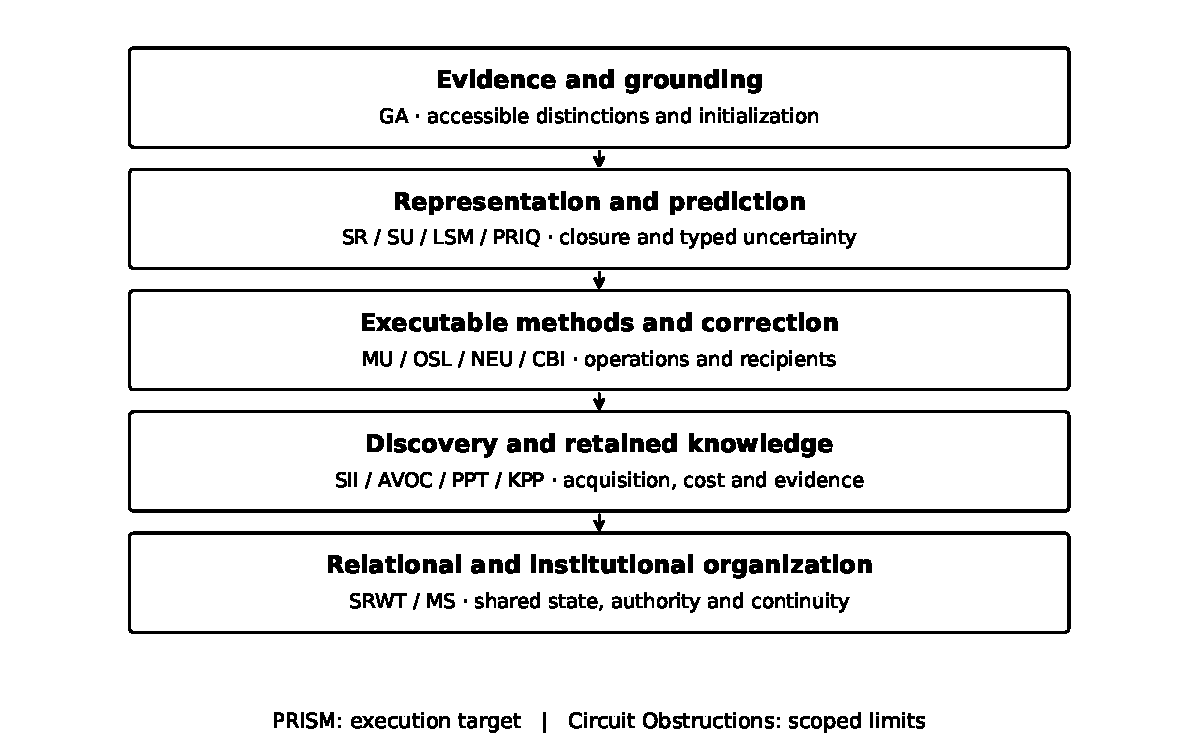
\includegraphics[width=\linewidth]{../figures/connected_layers.pdf}
\caption{The organizing structure. Arrows identify interfaces to be justified, not completed software integrations. Evidence and resource conditions remain relevant at every layer.}
\end{figure}

\section{A common contract, not a universal architecture}
For editorial purposes, write a task contract as
\[
\mathfrak C=(\Omega,\Pi,\mathcal Q,\mathcal A,\mathcal E,\mathcal B,\mathcal V).
\]
Here $\Omega$ is the declared family of possible worlds or models, $\Pi$ the permitted observation protocols, $\mathcal Q$ the protected questions, $\mathcal A$ the admitted actions or operations, $\mathcal E$ the evidence language, $\mathcal B$ the resource envelope, and $\mathcal V$ the validation and authority rules. This tuple is an editorial interface schema. It is not proposed as the unique primitive definition used by every source.

A realization of the contract may carry physical or computational state $x_t$, an observation history $h_t$, a retained predictive state $z_t$, a candidate set or probability record, an operator library, and applicable certificates. An institution adds offices, permissions, claims, resource rights, and revision procedures. The representation of one layer is not automatically the complete state of the others.

Three features of the schema matter. First, a target is stated before sufficiency is claimed. Second, protocols determine what information the system can actually obtain. Third, validation belongs to an explicit rule and authority boundary. None of these is supplied by an evocative name for a latent space.

A shared notation also exposes incompatibilities. One paper may use a finite deterministic world and another a finite probability model. One representation may be a set quotient while another is a linear map. One cost model counts complete tree records while another counts interpreter visits. Composition requires a declared translation of these meanings. Writing the same symbol in both papers is not such a translation.

\subsection{A packet is not automatically a belief}
In the algebraic sources, a packet can be a component selected by a projector or an address in a resolved family. Such a component may contain signed or complex values. A probability distribution has additional positivity and normalization requirements. An evidentiary packet may instead retain claims, dependencies, and unresolved conditions. These are related uses of decomposition, not identical mathematical types. Large Signal Model Foundations makes the probability-domain requirement explicit, and Stratified Universality retains different carriers unless a certified comparison is supplied. \src{LSM}\src{SU}

\subsection{A certificate is not automatically a fact about the world}
A mathematical proof, a checked finite witness, a successful interpreter replay, an integrity digest, and an observed performance comparison answer different questions. A digest can bind bytes to a record without establishing its premise. A formal proof can derive a property of an abstract program without establishing that a host execution refines that program. A risk bound can be valid under a likelihood model without proving that the model is adequate.

The compilation consequently uses source-specific assurance. AVOC and Certified Bayesian Inference retain their archived formal evidence. The newer books retain their prose proofs and bounded reference checks. No common label upgrades the weaker evidence to the stronger one. \src{AVOC}\src{AVL}\src{CBI}\src{CBL}\src{GA}

\parthead{PART II}{From experience to a usable method}
\section{Grounding begins with accessible distinctions}
Grounded Abstraction supplies the first link. A family of candidate systems can leave the full underlying realization unidentified while fixing every output that matters to the declared task. Conversely, each candidate system may individually admit a useful representation while the observer lacks enough information to initialize a common one. The source separates identification from a family of laws, certainty from one finite record, and the acquisition of executable predictive state. \src{GA}

Suppose a deterministic state space $X$ has admitted transformations $F_a$ and protected output $q$. Define
\[
x\sim y\quad\Longleftrightarrow\quad
q(F_wx)=q(F_wy)\quad\text{for every admitted finite word }w.
\]
The empty word is included. When the operation domain is invariant, this equivalence supports well-defined quotient updates. It identifies which distinctions are needed for all specified continuations, not which distinctions are needed to reproduce every hidden detail. This principle occurs in Sufficient Resolution, Machine Understanding, and Stratified Universality under their respective hypotheses. \src{SR}\src{MU}\src{SU}

The missing link is initialization. Let $r(x)$ be the observer's actual initial record. A quotient may exist mathematically while a decoder from $r(x)$ does not.

\begin{connection}[Evidence must initialize the predictive class]
Let $p:X\to X/{\sim}$ be the behavioral quotient above. There exists an initializer $i:r(X)\to X/{\sim}$ with $i(r(x))=p(x)$ for every $x$ if and only if
\[
r(x)=r(y)\quad\Longrightarrow\quad x\sim y.
\]
When this holds, the initialized quotient predicts every declared finite continuation using its induced updates.
\end{connection}
\begin{proof}
Necessity follows because a function has one value on an equal input. For sufficiency, assign $i(r(x))=p(x)$; the hypothesis makes the assignment independent of the representative $x$. The quotient update $\overline F_a(p(x))=p(F_ax)$ is well-defined because behavioral equivalence is preserved by prefixing an action. Induction on word length gives $pF_w=\overline F_wp$, and the output factors through $p$. Thus the initialized quotient returns the protected output after every word.
\end{proof}

This is an elementary restatement of the factorization and continuation arguments shared by the sources, not a new priority claim. It gives a precise connection between grounding and understanding: the desired predictive state must be reachable from evidence available to its user.

A noisy observation needs a different conclusion. Distinct candidate laws can assign positive probability to every finite record. In that case no finite record is an error-free identifier, although a probability update or confidence statement may be justified. Substituting a highly probable candidate for certain knowledge changes the contract. Grounded Abstraction retains that distinction and quantifies the resulting decision error in its final part. \src{GA}

\section{Archives, predictive states, and operator closure}
The signal program distinguishes an observation, an exact archive of that observation, and a state sufficient for prediction. A left-invertible analysis map preserves the accepted observation. It does not recover unmeasured properties of the external process. A smaller predictive state can discard part of the observation while preserving all relevant future outputs. An exact archive can still fail as an efficient predictive state if every use requires expensive reconstruction. \src{LSM}

For a linear map $C:X\to Z$ and a known operation $A:X\to X$, an induced operation $B$ satisfying $CA=BC$ exists precisely when $\kerop C$ is invariant under $A$, with the codomain restricted to the attained image if necessary. The condition says that two inputs collapsed by $C$ remain collapsed after the operation. If it fails, the discarded distinction can return through the retained state.

This failure has a concrete block form. In coordinates separating retained and hidden state,
\[
\begin{pmatrix}z_{t+1}\\u_{t+1}\end{pmatrix}
=
\begin{pmatrix}A&B\\C&D\end{pmatrix}
\begin{pmatrix}z_t\\u_t\end{pmatrix}.
\]
Even if $u_t$ has small norm, the effect $Bu_t$ may be large. Retaining less state is therefore not justified by omitted magnitude alone. A predictive error bound needs a sensitivity or propagation bound. Sufficient Resolution studies hidden-return defects and exact memory alternatives. Large Signal Model Foundations places those mechanisms inside its refinement and predictive-closure account. \src{SR}\src{LSM}

\subsection{One common quotient across uncertain dynamics}
Consider two possible linear realizations on $\mathbb R^3$,
\[
A_0=\begin{pmatrix}1&1&0\\0&1&0\\0&0&2\end{pmatrix},\qquad
A_1=\begin{pmatrix}1&1&0\\0&1&0\\1&0&3\end{pmatrix}.
\]
Let $p(x_1,x_2,x_3)=(x_1,x_2)$ and let the output be $q(x)=x_1$. Both operators satisfy
\[
pA_i=Gp,\qquad G=\begin{pmatrix}1&1\\0&1\end{pmatrix}.
\]
Consequently the output after $k$ operations is $x_1+kx_2$ for either fixed model. In this particular example it also holds for arbitrary switching, since the same local intertwining equation holds for both operations. The uncertain third-coordinate dynamics remain irrelevant to the protected output.

That switching conclusion must not be generalized to mere output agreement between fixed models. Grounded Abstraction separately exhibits the distinction: agreement of each fixed model's trajectories need not survive mixing their operators. A common quotient is the stronger premise used in the displayed example. \src{GA}

\section{From latent computation to an explicit language}
Neuralese and OSL are complementary, not competing definitions of machine language. Neuralese studies internal operations on latent state and the stability of their future behavior. OSL supplies an explicit intermediate language in which an operation's type, provenance, effect, and admissibility can be represented and checked. A producer need not use symbolic coordinates internally in order to communicate through such an interface. \src{NEU}\src{OSL}

For a common invariant domain, let $r:X\to Z$ encode the relevant state, let $G_a$ act on $Z$, and let $T:Z\to W$ translate that state into another representation with operations $H_a$. The desired equations are
\[
rF_a=G_ar,\qquad TG_a=H_aT.
\]
The first connects the source process to its representation. The second connects that representation to the recipient interface.

\begin{connection}[Two local bridges compose over finite continuations]
Assume the domains used by both equations are preserved under all admitted operations and that a protected output has the form $q=\bar q\,Tr$. Then, for every admitted finite word $w$,
\[
TrF_w=H_wTr,\qquad qF_w=\bar q\,H_wTr.
\]
\end{connection}
\begin{proof}
For one operation, $TrF_a=TG_ar=H_aTr$. The empty word gives the identity. Applying the one-operation relation successively proves the first equation by induction, and composing with $\bar q$ proves the second. Domain invariance ensures that every successive application is licensed.
\end{proof}

The result is a composition of already familiar intertwining arguments. It states exactly what would be preserved by a correct learned semantic bridge. It does not construct $r$ or $T$, authenticate causal use of the selected carrier, or bound the translator's complexity. Those remain separate obligations. A powerful interpreter that solves the problem after receiving a trivial label has not supplied a free representation of the source mechanism. Machine Understanding makes recipient programs and their installed information explicit for this reason. \src{MU}

\subsection{Why the bridge remains open}
The OSL source describes a checked finite interface based on declared tables. The Neuralese source distinguishes such exact compiled controls from learned latent implementations. Their coexistence supports a precise research question, not a claim that a general Neuralese-to-OSL compiler has been completed. The missing relation is a learned, causally adequate, continuation-preserving translator under explicit access and resource limits. \src{OSL}\src{NEU}

\parthead{PART III}{Correction, decisions, and knowledge}
\section{Prediction and correction must share a representation}
A state can be sufficient for its current prediction and insufficient for the interpretation of later evidence. This is one of the most important connections between the books. Machine Understanding asks when translation commutes with filtering candidate models. Grounded Abstraction identifies the information that future corrections require. PRIQ asks when fine prediction and Bayesian updating descend to a coarse interaction model. The signal foundations add the probability domain on which a learned operator can be interpreted as an update. \src{MU}\src{GA}\src{PRIQ}\src{LSM}

For exact candidate elimination, a current set $V\subseteq\Omega$ is corrected by $V\mapsto V\cap E$. If the target observation is $t(V)$, a future-correction signature records
\[
\Sigma(V)=\bigl(t(V\cap E)\bigr)_{E\in\mathcal E}.
\]
Under the source's closure hypotheses, this captures the distinctions needed to answer after every permitted filter. The empty set matters: recognizing that all candidates have been contradicted is part of a correct update, not an exceptional case to omit from the theorem. \src{GA}

For noisy evidence, target uncertainty and sensor uncertainty are not generally independent. Two priors can have the same separate marginals while producing different target posteriors after the same report. A useful compressed probability memory must preserve the association between target values and likelihood profiles whenever future evidence depends on that association. Grounded Abstraction constructs such exact memory and separately bounds finite quantization. \src{GA}

\subsection{A coarse prediction is not necessarily a coarse posterior}
In a finite Bayesian model, a coarse partition can preserve likelihood-based correction for every prior when the observation likelihood is constant within each coarse cell. A quotient of the transition dynamics alone does not ensure that property. Likewise, a signed packet decomposition can reconstruct a belief without each packet separately being a probability distribution. The coarse dynamics, update law, and positive domain must be checked together. \src{PRIQ}\src{LSM}

This produces a practical hierarchy of questions. Does the retained state preserve the desired output? Does it preserve the probabilities of later reports? Does it preserve the posterior update? Does the rounded implementation maintain the required accuracy through repeated updates? Does the result remain valid under changed likelihoods or a revised evidence language? These are related but different preservation contracts.

\section{From a probability record to an accountable decision}
Certified Bayesian Inference gives a particularly concrete bridge between a returned computational object and an inference statement. Its protected scope is one finite-dimensional Gaussian observation update with stated rational input factors and arithmetic conditions. Packet residuals, finite stopping, outward-rounded verification, and parameter enclosures concern the same returned approximation. A general sequential filter is a separate extension. \src{CBI}\src{CBL}

AVOC addresses a different layer: whether inspecting, constructing, checking, or deploying an artifact is justified under an explicit value and resource model. A correct artifact can be a poor investment. A high estimated probability of passing a checker is not a passed check. An honest operation log can still require a separate sampling argument before it supports calibration. \src{AVOC}\src{AVL}

The two branches should therefore be connected through a concrete interface: a named posterior or uncertainty object, a loss function, a permissible action set, a bound on numerical or representation error, and costs for the actual chosen course of action. An inferred probability does not itself grant authority to perform that action.

\begin{connection}[A common decision bound]
Let $\mu$ and $\widehat\mu$ be probability measures on the same finite candidate set with $\TV(\mu,\widehat\mu)\leq e$. Suppose true and approximate responses satisfy $d(y_\omega,\widehat y_\omega)\leq d_0$ for all retained candidates. If $\ell(a,y)\in[0,1]$ is $K$-Lipschitz in its second argument, then for every admissible action $a$,
\[
|R(a)-\widehat R(a)|\leq\eta:=\min\{1,e+Kd_0\},
\]
where $R(a)=\sum_\omega\mu_\omega\ell(a,y_\omega)$ and $\widehat R(a)=\sum_\omega\widehat\mu_\omega\ell(a,\widehat y_\omega)$. An action minimizing $\widehat R$ has regret at most $2\eta$ relative to a minimizer of $R$ when the action set is finite and nonempty.
\end{connection}
\begin{proof}
Insert the intermediate expectation $\sum\widehat\mu_\omega\ell(a,y_\omega)$. The first difference is at most $e$ because the integrand is in $[0,1]$. The second is at most $Kd_0$. Risks themselves lie in $[0,1]$, giving the cap. If $\widehat a$ and $a^*$ minimize the approximate and exact risks, respectively, then $R(\widehat a)\leq\widehat R(\widehat a)+\eta\leq\widehat R(a^*)+\eta\leq R(a^*)+2\eta$.
\end{proof}

This consolidates the elementary bound used in the quantitative grounding and decision work. It is a statement about one common posterior, response, history, and loss. It does not combine independently attractive bounds whose quantities refer to different candidate worlds. Nor does it imply a zero-risk guarantee from a small positive error. \src{GA}\src{MU}\src{AVOC}

\section{Mathematical memory is more than the final proof}
Proof Path Theory distinguishes a certificate of implication from the larger field of inquiry surrounding it. A valid proof can omit a useful failed route, a counterexample to a stronger claim, an alternative representation, or a dependency that explains how to adapt the argument. Retaining every exploration trace is not automatically optimal either. The source makes retention relative to future task families and recovery costs. \src{PPT}

This connects to corrective memory without identifying the two objects. A candidate-set signature preserves future filters under one finite evidence language. A proof field preserves specified routes of deduction, audit, and discovery. Both ask what compression makes unavailable, but they use different types of future operation. A shared storage implementation would need an explicit mapping between those operations.

The Preservation Protocol adds a temporal distinction. Earlier artifacts and recorded events remain recoverable, while present beliefs and authoritative pointers can change. Refuting a claim should not delete the fact that it was once asserted or the reason it was revised. That is a protocol for research continuity, not a proof that every surviving record is correct. \src{KPP}

The portable-lineage protocol extends the question to successor systems: does a bounded transferred state support correction retention, selective reuse, and resumed work? Its source is a protocol specification, not a completed demonstration of every proposed continuity level. It does not decide subjective identity. \src{PCL}

\parthead{PART IV}{Revision, shared work, and execution}
\section{Improving a method and improving its discovery}
Self-Improving Intelligence separates a solver, a procedure that constructs repairs, and the representation used to acquire rules inside that procedure. Its finite development includes diagnostic trees, certified compiler shortcuts, a grammar-synthesized pruning rule, a proof-checked equation library, and ordered quotienting that preserves the complete teacher transcript. Each acquired object is distinct from the supplied language and checker used to obtain it. \src{SII}

This makes a recursive step mathematically discussable without requiring that a system invent its own foundations. A descendant can be better at acquiring future rules because an acquired representation eliminates redundant search. Whether this is an end-to-end improvement depends on the cost of preparing and maintaining that representation and the workload over which it is reused.

SRIC is the larger historical theory behind this distinction. It contains repair transport, branching lineages, evaluator contexts, changing languages, and several conditional accounts of continued improvement. The 505-page source retains mathematical theory and experimental development together. It is preserved in the companion volume rather than silently replaced by the smaller first-edition book. Its historical results are not new evidence for a combined architecture. \src{SRIC}

\subsection{A correction should carry its reason for remaining valid}
A learned shortcut may depend on arithmetic semantics, a grammar order, a repair-success relation, an observation channel, or a resource comparison. A later change can leave the shortcut's printed expression unchanged while invalidating the justification for using it. The certificate-dependency construction in Self-Improving Intelligence marks the affected descendants and rechecks them under revised premises. \src{SII}

An unchanged theorem is not an unchanged application. If the repair language gains an action that succeeds in every case, an old lower bound based on identifying individual cases no longer describes the problem. The mathematical theorem remains true within its original scope. Its premise has stopped matching the revised system.

This is the connection to proof-path and preservation theory: a system should retain both the acquired method and the dependencies that determine its applicability. It is also the connection to OSL: admission should be tied to the actual operation and its current scope, not merely to an earlier approval string.

\section{A workspace is not yet a society}
SRWT studies compatible organization distributed across heterogeneous carriers. Its structural layer uses transfer maps, global compatible sections, and holonomy-fixed cores. Its dynamic and causal layers separately ask whether the proposed shared state predicts the relevant future, can be intervened on appropriately, remains reconstructible, and contributes beyond matched local alternatives. \src{SRWT}

These distinctions prevent two shortcuts. A synchronized collection of replicas is not necessarily irreducibly distributed cognition. Conversely, a state split into complementary shares by an external constructor does not by itself demonstrate endogenous organization. How the components are defined and what alternatives they are compared against belong to the claim.

Machine Societies adds rules that alter the space of permissible action: offices, membership, obligations, dispute procedures, resource allocation, and revision authority. A society can have several decision centers and no single global utility function. A coherent collective policy and persistent institutional plurality are separate properties. \src{MS}

The bridge from workspace to institution therefore requires more than a shared vector. A representation of a promise must connect to future obligations and remedies. A representation of a vote must connect to an electorate and a procedure. A shared archive must distinguish who can observe an event from who can authorize its consequences.

\subsection{Internal dynamics and external authority}
The Python Agent Dynamics atlas illustrates private candidate sets, messages, prediction discrepancies, and externally consequential actions in a finite model. It is a useful visual language for this interface, but its supplied update rules are not measured neural mechanisms. \src{AD}

In the theoretical compilation, an agent's internal confidence remains separate from the permission to act. An institutional acceptance rule does not establish another party's consent. A society can be internally consistent while omitting a legitimate external claim. The accountable-ending and external-effects material in Machine Societies prevents persistence from becoming its own unrestricted justification. \src{MS}

\section{Representation gains and execution costs}
PRISM studies a representation-aware execution architecture. Packet graphs, structured factors, sparse chains, and transform plans can remain explicit computational objects rather than being expanded into dense arrays by default. Packet IR makes representation, precision, schedule, and output contracts part of the compiler's decisions. The source preserves the distinction between software evidence and a proposed physical architecture. \src{PRISM}

This is downstream of the learning question. A system must obtain useful structure, verify its scope, and pay the costs of encoding and selecting it. A faster execution path for a supplied low-rank factorization is not an algorithm that discovers the factorization or proves that it is useful for an unfamiliar task.

Circuit Obstructions contributes a complementary limitation. Some proposed exact summaries must retain a large amount of structural information under their declared preservation rules. Some projections can destroy support properties or increase the relevant nonlinear cost. These are scoped complexity statements, not an unrestricted complexity-class separation. \src{CIR}

The combined lesson is neither that every representation change speeds computation nor that compression is futile. It is that the complete path must be accounted for:
\[
\text{acquire}\ \longrightarrow\ \text{represent}\ \longrightarrow\ \text{select}\ \longrightarrow\ \text{verify}\ \longrightarrow\ \text{execute}\ \longrightarrow\ \text{maintain}.
\]
The arrows can have different units. Model observations, interpreter visits, physical time, peak memory, and stored records should not be summed without an explicit conversion model.

\begin{connection}[Resource gains belong to a declared ledger]
For one fixed workflow and workload, let $\Delta\in\mathbb R^d$ be old-minus-new event counts after all charged setup and maintenance. Then $w^\top\Delta\geq0$ for every $w\in\mathbb R^d_{\geq0}$ if and only if every coordinate of $\Delta$ is nonnegative. For prices restricted to the convex hull of a finite set, the smallest priced saving is attained at one of its listed points.
\end{connection}
\begin{proof}
Nonnegative coordinates give a nonnegative scalar product. A negative coordinate is exposed by assigning positive price only to that coordinate. A linear functional at a convex combination is the same combination of its values, which cannot be below the smallest listed value. A listed minimizer attains that value.
\end{proof}

This restates the accounting principle in Self-Improving Intelligence. For its recorded weighted-search comparison, the vector $(1552,1552,-1868)$ counts saved model reads, saved additions, and added comparisons. Equal prices give a positive margin; other prices give a loss. Semantic validity does not change with that choice. Neither does a correct price calculation imply that the price is a measured property of a particular processor. \src{SII}

\begin{figure}[H]\centering
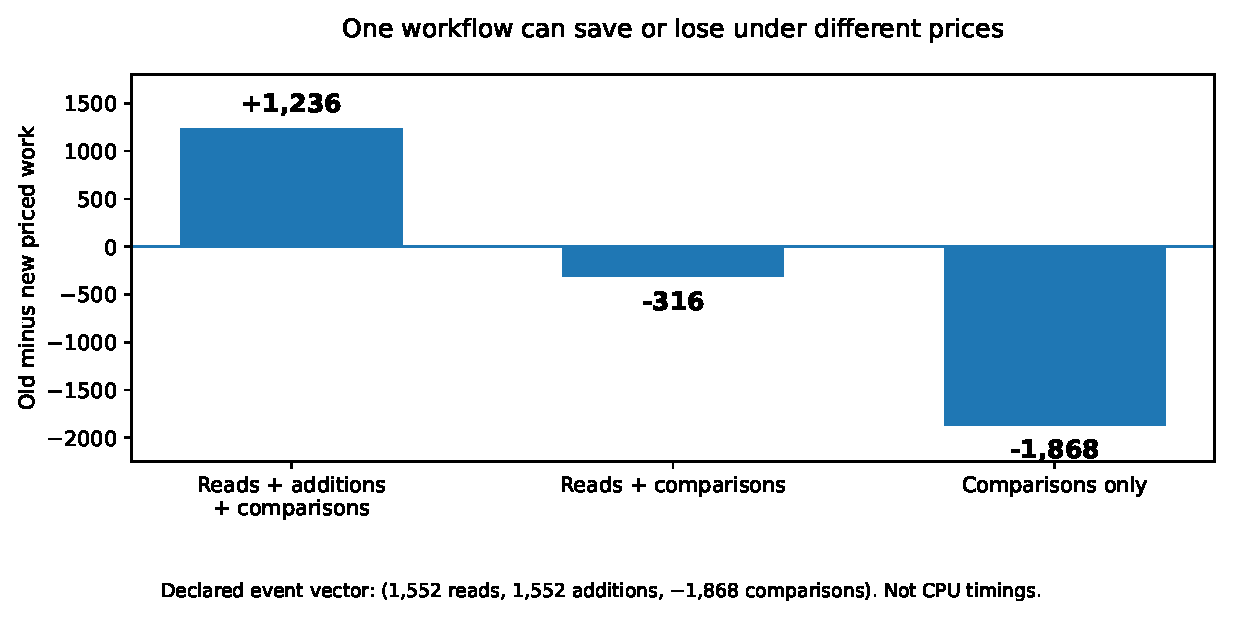
\includegraphics[width=0.95\linewidth]{../figures/resource_prices.pdf}
\caption{One source-reported event vector under three declared price assignments. Positive values are savings and negative values are losses. These are arithmetic consequences of the stated model, not runtime measurements.}
\end{figure}

\parthead{PART V}{One exact example through the whole chain}
\section{The sensor, the method, and the community}
The following construction is new editorial glue. It is not a claim that the implementations in all twenty-four sources share a common runtime. Its purpose is to make the interface obligations jointly inspectable in one small model.

Let the possible world be
\[
\omega=(b,\theta,u)\in\F_2^3.
\]
The bit $b$ determines which of two repairs is appropriate. The bit $\theta$ is a sensor convention. The nuisance bit $u$ affects none of the admitted observations, transitions, or repairs. A normal reading returns $s=b\oplus\theta$. A calibration returns $\theta$. A public operation flips $b$, leaving $\theta$ and $u$ unchanged. A repair $R_i$ succeeds precisely when $b=i$.

All of these semantics are stipulated. The small check program verifies the resulting finite claims. It does not learn the observation law, infer the truth of an external sensor model, or discover the repair meanings.

\subsection{First: a two-state predictor is enough for the display}
For the original question family, the task is only to predict the next display after a finite number of flips. The retained state $z=s$ has two possible values, and its update is $G(z)=1-z$. Every future display is determined even though $b$ and $\theta$ are not separately known. The nuisance bit is irrelevant throughout.

This is a direct illustration of the signal and sufficiency layers: lossless storage of the complete world is unnecessary for this prediction contract. It also illustrates grounding: the predictor can be initialized from the actual normal reading rather than from an inaccessible hidden bit.

\subsection{Second: the repair question changes the required distinction}
When the task becomes selecting $R_b$, the old display is insufficient. Worlds $(0,0,u)$ and $(1,1,u)$ have the same display and different successful repairs. Repeating the normal reading changes no information. Calibration supplies the missing convention, after which
\[
b=s\oplus\theta.
\]
The refinement is a genuine information acquisition. Merely adding a field named $\theta$ to the retained record would not initialize it.

If calibration is unavailable, no protocol built solely from the admitted flip and normal-reading operations can distinguish those two worlds. Their display histories remain the same after matched flips. Certain repair is therefore impossible within that unchanged interface. This is an interface-relative conclusion, not a claim that no richer experiment could help.

\subsection{Third: a translation can preserve the method}
One recipient stores $(s,\theta)$ and another stores $(b,\theta)$. The translator
\[
T(s,\theta)=(s\oplus\theta,\theta)
\]
is invertible. Both coordinate systems have a well-defined flip operation, and $T$ commutes with those operations. Both decode the same required repair. The exact correspondence gives an elementary realization of the method-transport contract.

The translator still has an access requirement and an execution cost. It cannot translate a record containing only $s$ into the missing pair. It does not infer a sensor convention from a matching variable name. This is the distinction between a valid map on its domain and a procedure that can obtain the map's input.

\begin{figure}[H]\centering
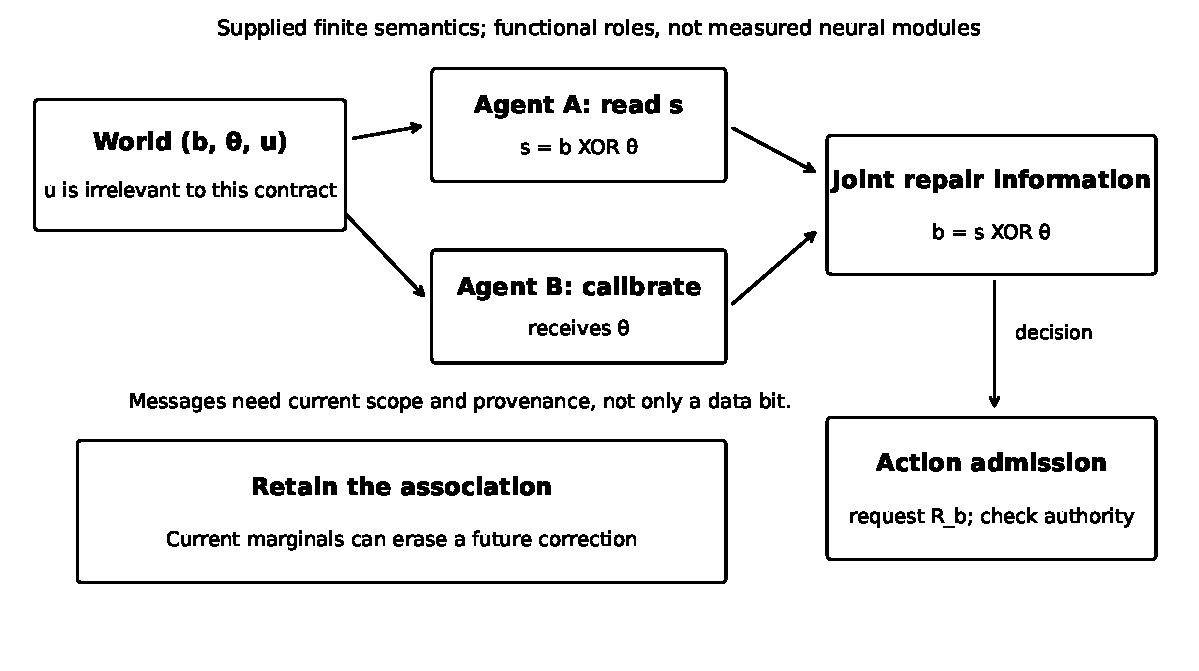
\includegraphics[width=\linewidth]{../figures/sensor_interfaces.pdf}
\caption{The same finite example through observation, calibration, coordinate transport, and checked action. The communication and authority conditions are additional interfaces, not consequences of the XOR identity.}
\end{figure}

\section{Memory, messages, and a changed task}
For candidate sets in the eight-world model, evidence depends only on $(b,\theta)$. There are four nonempty cells, each differing only in $u$. Restrict the evidence language to exactly the unions of those four cells. The occupancy record stores whether the current candidate set meets each cell. It therefore has $2^4=16$ possible states rather than the $2^8=256$ possible complete candidate sets.

That occupancy is sufficient to filter by every event in the declared evidence algebra and to return the possible target values $b$, including contradiction. It is also necessary across all candidate subsets for this contract. If two occupancies differ on one cell, filtering by that cell gives a nonempty target set in one case and the empty set in the other. This is the partition-evidence special case developed in Grounded Abstraction. \src{GA}

Four occupancy bits should not be confused with an exact probability record. When the model uses probabilities rather than possibilities, one needs the masses of the four joint cells, and storing those masses to arbitrary precision is a different resource problem. The source's finite quantization construction addresses that additional problem.

\subsection{Separate marginals can erase the next correction}
After display zero, the possible pairs are $(0,0)$ and $(1,1)$. After display one, they are $(0,1)$ and $(1,0)$. In both cases the separate target and sensor possibility sets are $\{0,1\}$. A memory retaining only those marginals identifies the two histories.

Now observe $\theta=0$. In the first history $b=0$, while in the second $b=1$. The same future evidence must lead to different corrections. The lost relation was not restored by the arrival of that evidence. Retaining the joint occupancy, or the relevant original display with its scope, avoids the error.

\subsection{Two agents and one action}
Let agent A obtain the normal reading and agent B obtain the calibration. Neither has the complete repair information alone. B can send its one-bit calibration result together with the declared provenance required by the communication protocol. Under truthful, correctly associated delivery, A can determine $b$ and request the correct repair.

This is shared information, not a theorem that the two agents form an endogenous workspace or a society. A workspace claim additionally needs the source's causal, persistence, and comparison conditions. An institutional claim needs an operative rule governing who may issue, verify, and execute the request. We can specify a rule that accepts a repair only when the current applicable records imply its success, but specifying it is not observing its spontaneous formation. \src{SRWT}\src{MS}

The data bit is also not the complete message cost. Provenance, episode association, delivery, and checking are separate components. The toy calculation treats the payload as one bit and leaves any metadata or transport overhead explicitly outside that number.

\subsection{Work and stored control}
Give a normal reading cost one, calibration cost two, and the final repair cost one, in stipulated work units. Certain repair from the complete initial uncertainty set requires both information channels, so the common worst-case work is four units. There are three primitive calls. Four weighted work units are not four calls.

A literal binary decision tree with these two observations and four outcome leaves contains seven records, although a run visits only three records. This is not the minimum size of every possible program encoding. A reusable arithmetic implementation is a different storage representation and must retain its own code and interpreter costs. The example illustrates the literal-tree convention used in the source books, rather than confusing it with a general description-length theorem. \src{MU}\src{SII}

\section{Revision can change the proof obligation}
Suppose a newly admitted repair $R_*$ succeeds for either value of $b$. Then the task no longer requires identifying $b$ before acting. The old statement that both information channels are necessary applied to the previous repair language. It does not apply after $R_*$ is introduced.

A well-formed revision record preserves the sensor identities and the old theorem while invalidating its application to the new task. The display predictor remains valid. The coordinate translator remains valid. The old minimum-information claim does not. A new controller can execute $R_*$ immediately under its declared cost and authority conditions. The old performance comparison must be recomputed if it referred to the former observation-and-repair workflow.

This single change connects all the levels: grounding is relative to future use; sufficiency is relative to the operation and target language; correction memory is relative to future evidence; procedure cost is relative to one actual algorithm; and certificate applicability is relative to current dependencies. \src{GA}\src{MU}\src{SII}

\begin{figure}[H]\centering
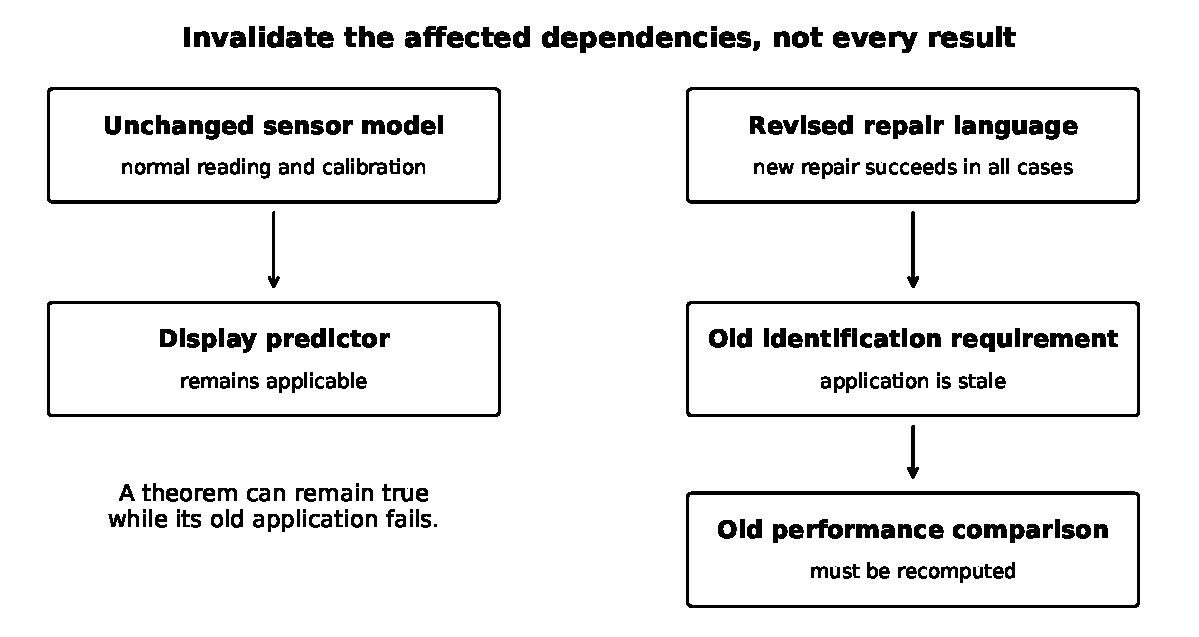
\includegraphics[width=\linewidth]{../figures/selective_invalidation.pdf}
\caption{A repair-language change need not invalidate the sensor semantics or display predictor. It does invalidate uses of the old identification requirement and dependent performance conclusions. This is a schematic dependency example, not a claim to infer complete dependencies automatically.}
\end{figure}

\subsection{What this example connects and what it does not}
The source theories can be instantiated on one common finite object with explicit maps. That is stronger than drawing an arbitrary chain of module names. It establishes neither a learned encoder nor a general-purpose system. Its sensor semantics, allowed actions, agents, message interpretation, and authority rule are supplied.



\parthead{PART VI}{The connection register and the research frontier}
\section{Which bridges are already mathematical?}
The register below distinguishes conditional mathematical connections from proposed integrations. ``Available'' means the source supplies a relevant theorem or construction under explicit premises. It does not mean every implementation in the two sources has been connected.

\small
\begin{longtable}{@{}p{0.08\linewidth}p{0.25\linewidth}p{0.57\linewidth}@{}}
\toprule ID & Interface & Required connection and present boundary\\\midrule\endhead
B01 & SR / SU to LSM & Available: typed decomposition and continuation-preserving transport. Packet completeness, kernels, profiles and admissible coefficient domains must match.\\
B02 & GA to MU & Available: accessible evidence initializes the distinctions needed by future use and correction. A quotient's existence does not supply its initializer.\\
B03 & LSM to GA & Available in specified models: observable prediction can avoid full-state identification. Candidate-model scope, probability validity and initialization remain explicit.\\
B04 & PRIQ to LSM / GA & Available: prediction and Bayesian correction descend under stated compatibility. Positivity, likelihood fibers and evidence normalization cannot be dropped.\\
B05 & Neuralese to OSL & Proposed learned bridge. A finite declared-table interface exists, but general causal, continuation-preserving learned translation is not established.\\
B06 & OSL to MU & Available as a contract: the actual typed recipient must execute the transmitted method within its own bounds. A decoder designed after the fact is a different contract.\\
B07 & GA / CBI to AVOC & Available conditionally: pass the same posterior object and its output error into a specified decision model. A one-observation Gaussian theorem does not imply a general sequential filter.\\
B08 & MU to SII & Available: acquisition, explanation and repair require one workflow satisfying its complete resource profile. Reusable methods and discovery procedures are different targets.\\
B09 & SII to OSL & Partial: both supply explicit admission obligations. A complete refinement proof linking all generated source forms to the runtime remains separate.\\
B10 & PPT / KPP to SII & Available at the specification level: retain dependencies, evidence and revision history. Dependency completeness and external premise adequacy are not inferred from hashes.\\
B11 & SRWT to MS & Additional hypotheses required: compatible shared state does not by itself create offices, authority, obligations or independent decision centers.\\
B12 & MS to SII & Available as an authority contract: an allowed local revision must preserve applicable institutional constraints. Formal capability does not authorize external control.\\
B13 & LSM to PRISM & Architecture path, not completed hardware: Packet IR must preserve the same typed output contract, numerical precision and costs.\\
B14 & CIR to discovery & Scoped limitation: exact summaries and projections face model-specific obstructions. No unrestricted computational separation follows.\\
B15 & Proof learner to action & Open integration in the recovered handoff: checked proof construction and the world-action dispatcher remain distinct branches.\\
B16 & Whole collection & No unrestricted composition theorem is claimed. One realization must satisfy all invoked interfaces simultaneously, with common evidence, costs and authority.\\\bottomrule
\end{longtable}
\normalsize

\section{Overlap is a reason to cross-reference, not inflate counts}
Several ideas recur because they do real work in different domains. The same elementary factorization criterion appears in task sufficiency, predictive initialization, and feature sufficiency for a synthesis decision. Induction extends local operation agreement to finite words. Bayesian normalization repeatedly introduces an evidence denominator. A dependency graph repeatedly exposes stale certificates. A resource vector repeatedly prevents gains in one unit from being promoted to a universal speedup.

Those recurrences should not be counted as independent discoveries solely because they occur in different books. They should also not be deleted before the scope differences are compared. A set-valued correction theorem is not automatically the same theorem as a stochastic posterior theorem. A fixed-model continuation result is not a switching-system result. A source-specific finite formalization is not a proof of every more general prose statement sharing its terminology.

The editorial consolidation therefore keeps one source edition per selected contribution and supplies overlap notes rather than removing proof bodies. The new connecting results in this synthesis are elementary restatements or direct compositions. Their role is to expose the interface assumptions, not to increase the portfolio's novelty count.

\subsection{Four different meanings of ``complete''}
An editorially complete manuscript has a frozen presentation and stated scope. A theorem complete under hypotheses has a valid derivation of its conditional conclusion. A verified implementation has an assurance record for the actual source and environment. An integrated learning system would instantiate the required objects and their acquisition mechanisms together. None of these meanings can be substituted for another by assigning the whole collection version 1.0.0.

The present version freezes a collection. Individual source numbers and open problems are retained. Large Signal Model Foundations remains at 0.4.0, OSL's runtime remains Core 0.5, and SRIC remains its historical Block 23 edition. The collection does not create a new release of those components.

\section{A theory-first agenda after the compilation}
The highest-value continuation is not another survey asserting that representations and memory matter. It is a short sequence of bridge problems with explicit mathematical endpoints.

\textbf{Evidence-limited semantic acquisition.} Determine which operation and representation claims can be identified from a restricted observation language, under model misspecification and changing tasks. Separate an unavailable distinction from an expensive one. The current finite and linear results supply starting cases, not a general learned encoder. \src{GA}\src{LSM}\src{NEU}

\textbf{State-changing noisy correction.} Join controlled stochastic realization with compressed probability memory and long-horizon correction. A static latent model, a dynamically changing hidden state, and an actively selected experiment do not have the same posterior recursion. The new bridge should specify common observation laws, probability domains, and conditioning margins before transporting finite-record bounds. \src{GA}\src{PRIQ}\src{LSM}

\textbf{Preserving a method when its learner changes.} Characterize what must be carried when encoders, operator libraries, recipient programs, and evidence languages are revised together. The target is not preserving every old answer. It is preserving justified operations and the means to correct an obsolete answer. \src{MU}\src{SII}\src{PPT}

\textbf{A small semantic core with a complete formal boundary.} Reuse the actual formal ingredients of AVOC and Certified Bayesian Inference where their domains fit. Identify a modest set of source-to-runtime preservation statements rather than promise a kernel proof for the entire archive. An abstract checker theorem and its host implementation remain distinct until their relation is proved. \src{AVOC}\src{AVL}\src{CBI}\src{CBL}\src{OSL}

\textbf{Discovery cost and changing languages.} Analyze classes where useful refinements or search quotients can be found economically, and classes where a compact solution exists but remains hard to acquire. Charge preparation, unsuccessful proposals and maintenance. A grammar extension can enlarge expressibility while reducing fixed-budget productivity. \src{SII}\src{CIR}

\textbf{Relational correction under plural authority.} Study when several agents can preserve shared meanings, independent evidence, and legitimate challenge while their representations and membership change. This is not solved by demanding consensus. It requires a common interface that distinguishes knowledge, action rights, and institutional obligations. \src{SRWT}\src{MS}

Each direction admits precise finite, algebraic, probabilistic, or analytic subproblems. Large-scale training is a possible later application, not a prerequisite for completing those theoretical results.

\section{Collection scope and the remaining source queue}
This edition includes twenty-four full source documents: ten core machine-theory works, seven mathematical and architectural foundations, and seven formal, visual, or lineage companions. Six existing editable source archives from the current development are included separately and unchanged. The compilation's own LaTeX, assembly code, figures, exact connecting-example checker, and catalogue are provided.

The standalone full source releases for many older library works were not collected in this pass. Their PDFs are included, but that is not a claim that their entire code, raw evidence, dependencies, or proof toolchains have been packaged. The source catalogue marks this explicitly.

Typed Proof Learner and Resolution Completion are represented by their recovered handoff note, not by a recovered merged implementation. Model-Theory Normalization, the broader Resolution Theory source families, RRCT/J-space experimental lineages, and task-specific ARC releases remain in the source-completion queue. Their absence from the unabridged reader is not a finding that they do not exist or lack substantive results. The general mathematical representation layer is represented here by SU, SR, and PRIQ. Historical empirical branches are not necessary premises for the new synthesis.

This is a substantial connected compilation, not an assertion that every machine-related file has been recovered. A future collection update should use a source-preservation map to add or replace a component. It should not select the largest version number across unrelated lineages or silently overwrite the original source's evidence boundary.

\section{Conclusion}
Operation Komorebi's machine work is most coherently read as a theory of knowledge-bearing computation under change. A representation identifies some distinctions and discards others. An operation makes those choices consequential. Evidence determines which descriptions can be initialized and corrected. A recipient must actually be able to use a communicated method. A discovery procedure must earn its cost. A revision must preserve the conditions under which its retained claims apply. A collective must add explicit relations of access, authority, obligation and continuity.

The connecting example shows that these obligations can be placed on one finite realization without confusing their roles. The source works develop them much further in their respective domains. Their relationship is therefore more substantial than a list of specialist modules, but more conditional than a claim that a complete general intelligence has been assembled.

The compilation's positive thesis is that representation, evidence, operations, correction, discovery, and institutional organization can be studied as related mathematical objects while keeping their distinctions intact. That is the organizing basis for the next theoretical results, and the reason to preserve the full source corpus alongside the synthesis.

\clearpage
\section*{Source catalogue and reading routes}
\addcontentsline{toc}{section}{Source catalogue and reading routes}
The catalogue records selected editions, not a global latest-version assertion. Page counts include each source's original cover, preliminaries, appendices and references. Complete source-page offsets are generated in \texttt{PAGE\_MAP.csv}. The master reader has document-entry cards and source-prefixed page labels. The separate original PDFs remain available in \texttt{sources/}.
{\small\setlength{\parskip}{3pt}\subsection*{Core machine theory}

\needspace{7\baselineskip}\hypertarget{cat:GA}{}\textbf{GA --- Grounded Abstraction}\par

1.0.0; 43 source pages.\par

Evidence, identifiable prediction, correction memory, and finite quantitative decisions. Prose proofs and source-reported exact illustrations; no kernel certificate or learned physical model.\par

\needspace{7\baselineskip}\hypertarget{cat:MU}{}\textbf{MU --- Machine Understanding}\par

1.0.0; 50 source pages.\par

Reusable representation, recipient-relative explanation, acquisition and joint resource feasibility. Prose proofs and bounded reference constructions; an operational account rather than an empirical understanding test.\par

\needspace{7\baselineskip}\hypertarget{cat:LSM}{}\textbf{LSM --- Large Signal Model Foundations}\par

Foundations 0.4.0 / software 2.3.0; 66 source pages.\par

Signal realizations, packets, predictive closure, observable models, and certified probability domains. Theory edition, not a new production runtime; probability validity, identification and empirical adequacy are distinct.\par

\needspace{7\baselineskip}\hypertarget{cat:OSL}{}\textbf{OSL --- Operator-Symbolic Language}\par

Research edition 1.0 / Core 0.5; 18 source pages.\par

Typed operations, semantic checkpoints, provenance, bounded discovery and admission. Executable finite interfaces are described; complete interpreter soundness and general learned production are not established.\par

\needspace{7\baselineskip}\hypertarget{cat:NEU}{}\textbf{NEU --- Neuralese}\par

Research edition 1.0; 20 source pages.\par

Latent operator semantics, observable continuation, gauge and stability boundaries. Mixed theory and retained research history. Historical outcomes are preserved, not used as evidence for a combined agent.\par

\needspace{7\baselineskip}\hypertarget{cat:CBI}{}\textbf{CBI --- Certified Bayesian Inference}\par

Core 1.0.0 / standardized publication; 36 source pages.\par

One-observation Gaussian inference, packet residuals and outward-rounded output guarantees. Archived formal evidence is scoped to the stated construction; no new Lean run or general sequential filter is claimed here.\par

\needspace{7\baselineskip}\hypertarget{cat:AVOC}{}\textbf{AVOC --- AVOC: Artifact Value and Guarded Planning}\par

Formal 0.41.0 / standardized publication; 37 source pages.\par

Task sufficiency, guarded planning, calibration, artifact identity and operation lifecycle. Exposition of a formal archive; archived kernel evidence is not a fresh proof run by this compilation.\par

\needspace{7\baselineskip}\hypertarget{cat:PPT}{}\textbf{PPT --- Proof Path Theory}\par

1.0.0; 34 source pages.\par

Justification hypergraphs, certificate extraction, recovery debt and mathematical memory. Finite declared proof fields and written arguments; discovery memory is not itself a proof of its target.\par

\needspace{7\baselineskip}\hypertarget{cat:SII}{}\textbf{SII --- Self-Improving Intelligence}\par

1.0.0; 60 source pages.\par

Repair synthesis, compiler revision, acquired equations, certificate dependencies and resource prices. Bounded constructive chain with prose proofs; no indefinite recursive acceleration or unrestricted agent is inferred.\par

\needspace{7\baselineskip}\hypertarget{cat:MS}{}\textbf{MS --- Machine Societies}\par

1.0.0; 106 source pages.\par

Persistent plural organization, institutions, common policies, authority and accountable endings. Conditional theoretical models; internal coherence does not confer external legitimacy or demonstrate endogenous societies.\par

\subsection*{Mathematical and architectural foundations}

\needspace{7\baselineskip}\hypertarget{cat:SU}{}\textbf{SU --- Stratified Universality for Resolved Representations}\par

Mathematical base 2.0.0 / standardized publication; 262 source pages.\par

Typed representation transport, semantic quotients, carrier changes and profiled descent. Relative to declared grammars, profiles and bridges; not equivalence of all mathematical carriers.\par

\needspace{7\baselineskip}\hypertarget{cat:SR}{}\textbf{SR --- Sufficient Resolution}\par

Standardized publication; 47 source pages.\par

Behavioral sufficiency, hidden-return memory, reconstruction, regularization and calibration. Preserves source-specific prose and archived formal distinctions; hypotheses are not supplied by the reader.\par

\needspace{7\baselineskip}\hypertarget{cat:PRIQ}{}\textbf{PRIQ --- Hypergraph Lumpability and Bayesian Refinement}\par

0.1.4; 52 source pages.\par

Nonlinear interaction quotients, prediction and update compatibility, posterior and pruning defects. Mathematical refinement contracts with exact and numerical illustrations; no universal learned quotient.\par

\needspace{7\baselineskip}\hypertarget{cat:SRWT}{}\textbf{SRWT --- Stratified Relational Workspace Theory}\par

209-page monograph / repository 1.0.0; 209 source pages.\par

Compatible shared cores, causal relevance, persistence, reconstruction, identity and decomposition. A workspace specification and theory; structural gluing alone does not establish causal efficacy or institutional agency.\par

\needspace{7\baselineskip}\hypertarget{cat:CIR}{}\textbf{CIR --- Circuit Obstructions}\par

Standardized publication / Lean Block 02 scope; 35 source pages.\par

Restored reversible computation, complete covers and limits of exact projection. Scoped circuit and representation bounds; not a general superpolynomial separation or SAT solver.\par

\needspace{7\baselineskip}\hypertarget{cat:PRISM}{}\textbf{PRISM --- PRISM-1: Packet-Programmable Processing}\par

Final updated architecture draft; 61 source pages.\par

Packet IR, mixed representations, structured scheduling and reconstruction contracts. Architecture specification with separately retained software evidence; not fabricated or fully qualified hardware.\par

\needspace{7\baselineskip}\hypertarget{cat:KPP}{}\textbf{KPP --- Komorebi Preservation Protocol}\par

Specification draft 0.1; 20 source pages.\par

Immutable artifacts, revisable claims, provenance and recoverable continuation. Protocol specification, not proof that the entire archive already implements it.\par

\subsection*{Formal, visual, and lineage companions}

\needspace{7\baselineskip}\hypertarget{cat:AVL}{}\textbf{AVL --- AVOC: Lean and Evidence Companion}\par

Formal 0.41.0 / standardized publication; 44 source pages.\par

Declaration-level route from mathematical exposition to retained formal evidence. Formal-source guide; archival build records are not rerun in this compilation.\par

\needspace{7\baselineskip}\hypertarget{cat:CBL}{}\textbf{CBL --- Certified Bayesian Inference: Lean Companion}\par

Core 1.0.0 / standardized publication; 31 source pages.\par

Source-level contracts, archived kernel evidence and one-observation solver proofs. The formal scope remains one observation update under exact stated model assumptions.\par

\needspace{7\baselineskip}\hypertarget{cat:SIV}{}\textbf{SIV --- Self-Improving Intelligence: Visual Guide}\par

1.0.0; 36 source pages.\par

Visual route through repair, discovery, search acquisition and changing guarantees. Expository companion; neither new learning evidence nor a replacement for the proofs.\par

\needspace{7\baselineskip}\hypertarget{cat:AD}{}\textbf{AD --- Agent Dynamics: Python Visual Atlas}\par

1.0; 14 source pages.\par

Internal beliefs, evidence exchange, revision and external action in an explicit finite model. Rule-based illustrative dynamics, not measured neural modules or learned self-improvement.\par

\needspace{7\baselineskip}\hypertarget{cat:LSV}{}\textbf{LSV --- Large Signal Model: Visual Notes}\par

0.4.0; 9 source pages.\par

Seven mathematical views of certified probability domains and approximation. Analytical illustrations tied to LSM propositions; no task-suite or integrated-model claim.\par

\needspace{7\baselineskip}\hypertarget{cat:PCL}{}\textbf{PCL --- Portable Causal Lineage}\par

Protocol 0.2; 64 source pages.\par

Explicit functional continuity, correction retention and model-replacement tests. Preserved protocol design, not a completed implementation or established subjective continuity.\par

\needspace{7\baselineskip}\hypertarget{cat:SRIC}{}\textbf{SRIC --- Stratified Recursive Improvement Closure}\par

2.4 / Block 23; 505 source pages.\par

Extended repair theory, semantic transport, evaluator contexts and historical lineages. Mixed theoretical and historical monograph preserved in full. Historical claims are not replayed or imported as integrated evidence.\par}

\clearpage
\section*{Notation crosswalk}
\addcontentsline{toc}{section}{Notation crosswalk}
\begin{longtable}{@{}p{0.18\linewidth}p{0.72\linewidth}@{}}
\toprule Object & How it is used in the compilation\\\midrule
Representation & A specified map or retained object, relative to future queries and operations. It is not assumed lossless.\\
Packet & A typed component in a decomposition. Linear, probabilistic, evidentiary and institutional carriers are not identified by their shared name.\\
Transfer & A declared correspondence preserving named structure. A map can preserve outputs without preserving acquisition, authorization, or cost.\\
Residual & A discrepancy relative to a contract. A residual identifies failure of a conjunction, not necessarily its unique cause.\\
Closure & Preservation under a specified operation family. This is distinct from proof completeness, probability validity and open-ended discovery.\\
Correction & A justified change to retained candidates, probabilities, methods or claims. Historical records need not be erased.\\
Certificate & Evidence for a named statement under specified premises. Its assurance type and current applicability remain explicit.\\
Workspace & A relational organization satisfying the declared structural, predictive, causal and continuity conditions. Shared storage alone is insufficient.\\
Institution & Operative permissions, offices, commitments and revision rules among decision centers. Structural compatibility does not supply external consent.\\
Improvement & A gain under a stated comparison, including relevant installed information and costs. Editing, selection and gain are different events.\\\bottomrule
\end{longtable}

\section*{Assembly and review boundary}
\addcontentsline{toc}{section}{Assembly and review boundary}
The original PDFs and included source archives are copied byte-for-byte into the package. Source pages in the merged readers are compared with the originals for extracted text and geometry. Sampled source pages are also compared as rendered images. New covers, source-entry pages, and this synthesis receive separate visual review. These are preservation and publication checks, not a new proof review of approximately two thousand source pages.

The exact connecting-example checks use finite sets, integers and rational arithmetic. They test the stated eight-world model, translator, correction memory, common observable quotient, and resource calculations. They are not empirical observations about neural systems. The inherited research suites and Lean projects are not rerun. The complete validation scope, encountered failures, hashes, and source-preservation results are recorded in the collection review report.

No standalone font files, private conversation transcript, or third-party full research paper is added by the assembly. Existing source-specific licensing remains unchanged. The package is a working collection, not a blanket relicensing or a claim of external publication acceptance.
\end{document}
